\documentclass[theme=teal]{khmermath}
\usepackage{needspace}
\geometry{left=0.85cm, right=0.85cm, top=0.70cm, bottom=1.35cm, footskip=0.65cm}
\usepackage{colortbl}
\usepackage{tikz}
\usetikzlibrary{calc,shapes,arrows,intersections,through,backgrounds,shadows,decorations.pathmorphing}

% Define arc accent
\newcommand{\wideparen}[1]{\overset{\boldsymbol{\frown}}{#1}}

% -------------------------------------------------------------------------
% Korean Math Textbook Style Color Palette & Macros
% -------------------------------------------------------------------------
\definecolor{koreaTeal}{RGB}{0, 150, 155}       % Primary Header Teal/Cyan
\definecolor{koreaDarkTeal}{RGB}{0, 105, 110}   % Dark Teal Accent
\definecolor{koreaBeige}{RGB}{247, 244, 237}     % Concept Sidebar Beige
\definecolor{koreaBeigeBorder}{RGB}{225, 218, 205}
\definecolor{koreaOrange}{RGB}{235, 115, 30}     % Problem Number Orange
\definecolor{koreaBlue}{RGB}{35, 110, 190}      % Standard Blue
\definecolor{koreaPurple}{RGB}{125, 50, 160}    % Purple Accent
\definecolor{koreaNumber}{RGB}{115, 125, 135}   % Problem Number Gray
\definecolor{koreaYellow}{RGB}{255, 246, 175}   % Yellow Highlight Tint

\definecolor{brandNavy}{RGB}{0, 105, 110}
\definecolor{brandBlue}{RGB}{0, 150, 155}
\definecolor{brandLightBlue}{RGB}{247, 244, 237}
\definecolor{brandCrimson}{RGB}{195, 35, 60}
\definecolor{brandCoral}{RGB}{235, 80, 75}
\definecolor{brandGold}{RGB}{215, 130, 10}
\definecolor{brandGoldBg}{RGB}{255, 252, 242}
\definecolor{brandTeal}{RGB}{0, 150, 155}
\definecolor{brandTealBg}{RGB}{244, 252, 250}
\definecolor{subtleGray}{RGB}{246, 251, 249}
\definecolor{cardBorder}{RGB}{220, 212, 198}
\definecolor{treeGreen}{RGB}{34, 139, 34}
\definecolor{treeBrown}{RGB}{139, 69, 19}

% Custom Header & Footer setup (Korean Textbook Style)
\usepackage{fancyhdr}
\pagestyle{fancy}
\fancyhf{}
\renewcommand{\headrulewidth}{0pt}
\renewcommand{\footrule}{\color{koreaTeal!60}\hrule height 0.6pt\vspace{2.5pt}}

\fancyfoot[L]{%
  \fontsize{8.5}{8.5}\selectfont\kml \color{koreaNumber}\textbf{\thepage}\ \vline\ \color{koreaDarkTeal}\textbf{១៥. ទ្រឹស្ដីបទពីតាលែស}%
}
\fancyfoot[C]{%
  \fontsize{8.5}{8.5}\selectfont\kby \color{koreaDarkTeal}\textbf{\ding{72}\ បង្រៀនដោយ ៖ \textcolor{koreaDarkTeal}{ក្រូត រស្មី}\ \ding{72}}%
}
\fancyfoot[R]{%
  \fontsize{8.5}{8.5}\selectfont\kby \color{koreaDarkTeal}\textbf{ Telegram: \textcolor{brandCrimson}{070897540}}\ \vline\ \color{koreaNumber}\textbf{\thepage}%
}

% Korean Header Banner
\newcommand{\koreanheader}[2]{%
  \noindent%
  \begin{tikzpicture}[x=1cm, y=1cm]
    \fill[koreaTeal, rounded corners=12pt] (0, 0.1) -- (0, 0.95) -- (3.8, 0.95) [rounded corners=0pt] -- (4.4, 0.1) -- cycle;
    \node[white, font=\fontsize{11}{11}\selectfont\kml\bfseries] at (1.9, 0.52) {#1};
    \node[anchor=west, font=\fontsize{17}{17}\selectfont\kml\bfseries, color=koreaDarkTeal] at (4.6, 0.42) {#2};
    \node[anchor=east, font=\fontsize{8.5}{8.5}\selectfont\kby, color=gray!80] at (19.2, 0.48) {$>$ ក្លឹបសិក្សាគណិតវិទ្យា ភី ស៊ី​ អឹម};
  \end{tikzpicture}%
  \vspace{2pt}%
}

% Yellow Formula Highlight Box
\newcommand{\koreahl}[1]{\colorbox{koreaYellow}{\fontsize{8.5}{8.5}\selectfont\textbf{#1}}}

% General Rule Box (Teal/Emerald Theme - ជាទូទៅ)
\newtcolorbox{khboxorange}[1][]{
  enhanced,
  colframe=brandNavy!40,
  colback=brandLightBlue,
  boxrule=0.7pt,
  arc=4.5pt,
  borderline west={3.5pt}{0pt}{brandNavy},
  drop fuzzy shadow=brandNavy!15,
  left=8pt, right=8pt, top=5pt, bottom=4pt,
  title={\fontsize{9}{9}\selectfont\kml\color{white}\ding{72}\ ជាទូទៅ},
  coltitle=white,
  colbacktitle=brandNavy,
  boxed title style={
    boxrule=0pt,
    arc=3pt,
    left=6pt, right=6pt, top=2pt, bottom=2pt
  },
  attach boxed title to top left={yshift*=-\tcboxedtitleheight/2, xshift=10pt},
  #1
}

% Concept / Card Item Box
\newtcolorbox{khcard}[1][]{
  enhanced,
  colframe=cardBorder,
  colback=white,
  boxrule=0.6pt,
  arc=3.5pt,
  left=5pt, right=5pt, top=3.5pt, bottom=3.5pt,
  #1
}

% Section, Subsection & Header Badge Macros
\newcommand{\khsection}[2]{%
  \Needspace*{3.0cm}%
  \vspace{3pt}%
  \noindent%
  \begin{tikzpicture}
    \fill[rounded corners=4pt, brandNavy!7] (0,0) rectangle (19.3, 0.64);
    \fill[rounded corners=3pt, brandNavy] (0.05, 0.05) rectangle (0.58, 0.59);
    \node[white, font=\fontsize{9.5}{9.5}\selectfont\bfseries] at (0.32, 0.32) {#1};
    \fill[brandGold, rounded corners=1pt] (0.68, 0.13) rectangle (0.72, 0.51);
    \node[anchor=west, font=\fontsize{11}{11}\selectfont\kml, color=brandCrimson] at (0.78, 0.32) {\textbf{#2}};
  \end{tikzpicture}%
  \vspace{2pt}%
}

\newcommand{\khsubsection}[2]{%
  \Needspace*{2.5cm}%
  \vspace{3pt}%
  \noindent%
  \begin{tikzpicture}[baseline=(sub.base)]
    \node[rounded corners=3pt, fill=brandBlue!12, draw=brandBlue!35, line width=0.5pt, text=brandNavy, font=\fontsize{8.5}{8.5}\selectfont\kml\bfseries, inner sep=2.5pt] (sub) at (0,0) {#1};
    \node[anchor=west, font=\fontsize{9.5}{9.5}\selectfont\kml\bfseries, color=brandNavy] at (sub.east) {\ \ #2};
  \end{tikzpicture}%
  \vspace{1pt}%
}

\def\splitnum#1#2{%
  \color{koreaNumber!65}#1\color{koreaOrange}#2%
}
\newcommand{\koreannum}[1]{%
  \ifstrempty{#1}{}{%
    \mbox{%
      \fontsize{18}{18}\selectfont\bfseries%
      \ifnum#1<10\relax%
        \color{koreaNumber!65}0\color{koreaOrange}#1%
      \else%
        \expandafter\splitnum#1%
      \fi%
    }\,\ %
  }%
}

% Khmer Sub-item Badge (ក, ខ, គ)
\newcommand{\khlabel}[1]{%
  \tikz[baseline=-0.6ex]{%
    \node[fill=brandCrimson, rounded corners=2.8pt, inner sep=2pt, minimum width=1.3em, minimum height=1.28em, text=white, font=\kml\fontsize{7.5}{7.5}\selectfont, align=center] (lbl) {\raisebox{0.2pt}{#1}};%
  }\,\ %
}
\newcommand{\exhead}[1]{\hangindent=22pt\hangafter=1\koreannum{#1}}

\setlength{\parindent}{0pt}
\setlength{\parskip}{2.5pt}
\setlength{\columnsep}{16pt}
\setlength{\columnseprule}{0.5pt}
\def\columnseprulecolor{\color{koreaTeal!40}}

\begin{document}

% =========================================================================
% PAGE 1: ផ្នែកទី ១ ៖ បន្ទាត់ស្របនិងខ្នាត់
% =========================================================================
\koreanheader{មេរៀនទី ១៥}{ទ្រឹស្ដីបទពីតាលែស}

\khsection{១}{បន្ទាត់ស្របនិងខ្នាត់}

\begin{khboxorange}
  \begin{minipage}[c]{0.66\textwidth}
    \begin{itemize}[leftmargin=12pt, itemsep=2.5pt, topsep=1pt, parsep=0pt]
      \item[\color{brandNavy}\ding{228}] \textbf{បើបន្ទាត់ស្របកំណត់នៅលើខ្នាត់មួយបានអង្កត់ប៉ុនគ្នា នោះវាកំណត់នៅលើខ្នាត់ផ្សេងទៀតក៏បានអង្កត់ប៉ុនគ្នាដែរ ។}
      \item[\color{brandCrimson}\ding{228}] គេមានបន្ទាត់ស្រប $l_1 \parallel l_2 \parallel l_3$ កាត់ខ្នាត់ $d_1$ ត្រង់ $A, B, C$ និងកាត់ខ្នាត់ $d_2$ ត្រង់ $A', B', C'$ ៖
      \begin{equation*}
        \koreahl{$AB = BC \implies A'B' = B'C'$}
      \end{equation*}
    \end{itemize}
  \end{minipage}\hfill
  \begin{minipage}[c]{0.32\textwidth}
    \centering
    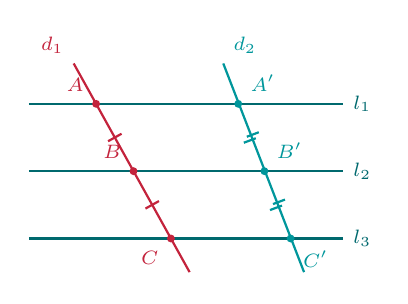
\begin{tikzpicture}[scale=0.95]
      % Parallel lines
      \draw[thick, color=brandNavy] (-1.9, 1.8) -- (2.3, 1.8) node[right, font=\fontsize{7.5}{7.5}\selectfont] {$l_1$};
      \draw[thick, color=brandNavy] (-1.9, 0.9) -- (2.3, 0.9) node[right, font=\fontsize{7.5}{7.5}\selectfont] {$l_2$};
      \draw[thick, color=brandNavy] (-1.9, 0.0) -- (2.3, 0.0) node[right, font=\fontsize{7.5}{7.5}\selectfont] {$l_3$};
      
      % Transversals d1 and d2
      \draw[thick, color=brandCrimson] (-1.3, 2.34) node[above left, font=\fontsize{7.5}{7.5}\selectfont] {$d_1$} -- (0.25, -0.45);
      \draw[thick, color=brandBlue] (0.7, 2.34) node[above right, font=\fontsize{7.5}{7.5}\selectfont] {$d_2$} -- (1.78, -0.45);
      
      % Points
      \coordinate (A) at (-1.0, 1.8);
      \coordinate (B) at (-0.5, 0.9);
      \coordinate (C) at (0.0, 0.0);
      \coordinate (Ap) at (0.9, 1.8);
      \coordinate (Bp) at (1.25, 0.9);
      \coordinate (Cp) at (1.6, 0.0);
      
      \fill[brandCrimson] (A) circle (1.5pt) node[above left=1pt, font=\fontsize{7.5}{7.5}\selectfont] {$A$};
      \fill[brandCrimson] (B) circle (1.5pt) node[above left=1pt, font=\fontsize{7.5}{7.5}\selectfont] {$B$};
      \fill[brandCrimson] (C) circle (1.5pt) node[below left=1pt, font=\fontsize{7.5}{7.5}\selectfont] {$C$};
      
      \fill[brandBlue] (Ap) circle (1.5pt) node[above right=1pt, font=\fontsize{7.5}{7.5}\selectfont] {$A'$};
      \fill[brandBlue] (Bp) circle (1.5pt) node[above right=1pt, font=\fontsize{7.5}{7.5}\selectfont] {$B'$};
      \fill[brandBlue] (Cp) circle (1.5pt) node[below right=1pt, font=\fontsize{7.5}{7.5}\selectfont] {$C'$};
      
      % Single ticks for AB = BC
      \draw[thick, color=brandCrimson] ($(-0.75, 1.35)+(-0.09, -0.05)$) -- ($(-0.75, 1.35)+(0.09, 0.05)$);
      \draw[thick, color=brandCrimson] ($(-0.25, 0.45)+(-0.09, -0.05)$) -- ($(-0.25, 0.45)+(0.09, 0.05)$);
      
      % Double ticks for A'B' = B'C'
      \draw[thick, color=brandBlue] ($(1.075, 1.35)+(-0.08, -0.03)+(0.02, 0.04)$) -- ($(1.075, 1.35)+(0.08, 0.03)+(0.02, 0.04)$);
      \draw[thick, color=brandBlue] ($(1.075, 1.35)+(-0.08, -0.03)+(-0.02, -0.04)$) -- ($(1.075, 1.35)+(0.08, 0.03)+(-0.02, -0.04)$);
      \draw[thick, color=brandBlue] ($(1.425, 0.45)+(-0.08, -0.03)+(0.02, 0.04)$) -- ($(1.425, 0.45)+(0.08, 0.03)+(0.02, 0.04)$);
      \draw[thick, color=brandBlue] ($(1.425, 0.45)+(-0.08, -0.03)+(-0.02, -0.04)$) -- ($(1.425, 0.45)+(0.08, 0.03)+(-0.02, -0.04)$);
    \end{tikzpicture}
  \end{minipage}
\end{khboxorange}

\vspace{1pt}
\begin{khcard}
  \begin{minipage}[c]{0.63\textwidth}
    {\bfseries\color{brandCrimson}\ding{70}\ ឧទាហរណ៍ ៖} គេមានអង្កត់ $AB$ មួយ ។ ចូរក្រិតអង្កត់ $AB$ ជាបីផ្នែកប៉ុនគ្នា ។\\[2pt]
    {\bfseries\color{koreaDarkTeal}\ding{45}\ ចម្លើយ ៖} ដោយគេពុំអាចប្រើម៉ែត្រដើម្បីក្រិត $AB$ ជាបីឯកតាបាន នោះគេត្រូវ ៖
    \begin{itemize}[leftmargin=10pt, itemsep=1.5pt, topsep=1pt, parsep=0pt]
      \item សង់បន្ទាត់ $Ax$ ដោយប្រើម៉ែត្រដើម្បីក្រិតនៅលើកន្លះបន្ទាត់ $Ax$ ឱ្យបានជាបីចំណែកប៉ុនគ្នាកំណត់ដោយចំណុច $C, D$ និង $E$ ។
      \item ភ្ជាប់ $BE$ រួចគូសបន្ទាត់ចេញពីចំណុច $D$ និង $C$ ឱ្យស្រប $(EB)$ កាត់បន្ទាត់ $AB$ ត្រង់ $D'$ និង $C'$ ។
      \item យើងបាន \koreahl{$AC' = C'D' = D'B$} ។ ធ្វើយ៉ាងនេះមានន័យថាគេបានក្រិត $AB$ ជាបីផ្នែកប៉ុនគ្នា ។
    \end{itemize}
  \end{minipage}\hfill
  \begin{minipage}[c]{0.35\textwidth}
    \centering
    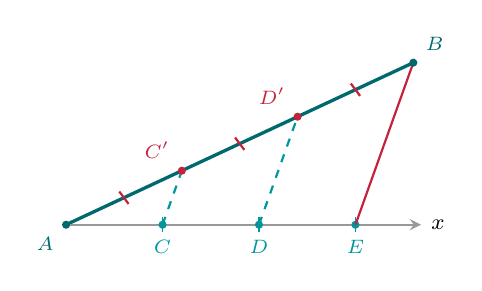
\begin{tikzpicture}[scale=0.98]
      \coordinate (A) at (0, 0);
      \coordinate (B) at (4.5, 2.1);
      \coordinate (C) at (1.25, 0);
      \coordinate (D) at (2.50, 0);
      \coordinate (E) at (3.75, 0);
      \coordinate (X) at (4.6, 0);
      
      % Segments AB and Ray Ax
      \draw[very thick, color=brandNavy] (A) -- (B);
      \draw[thick, color=gray!80, ->, >=stealth] (A) -- (X) node[right, font=\fontsize{8}{8}\selectfont, color=black] {$x$};
      
      % Ruler graduation ticks on Ax
      \foreach \pt in {C, D, E} {
        \draw[color=brandBlue, line width=0.6pt] ($(\pt)+(0,-0.10)$) -- ($(\pt)+(0,0.10)$);
      }
      
      % Points C, D, E
      \fill[brandBlue] (C) circle (1.5pt) node[below=2pt, font=\fontsize{7.5}{7.5}\selectfont] {$C$};
      \fill[brandBlue] (D) circle (1.5pt) node[below=2pt, font=\fontsize{7.5}{7.5}\selectfont] {$D$};
      \fill[brandBlue] (E) circle (1.5pt) node[below=2pt, font=\fontsize{7.5}{7.5}\selectfont] {$E$};
      
      % Line EB
      \draw[thick, color=brandCrimson] (E) -- (B);
      
      % Intersections C' and D' on AB
      \coordinate (Cp) at (1.5, 0.7);
      \coordinate (Dp) at (3.0, 1.4);
      
      % Parallel lines CC' and DD'
      \draw[thick, dashed, color=brandTeal] (C) -- (Cp);
      \draw[thick, dashed, color=brandTeal] (D) -- (Dp);
      
      % Points on AB
      \fill[brandNavy] (A) circle (1.5pt) node[below left=1pt, font=\fontsize{7.5}{7.5}\selectfont] {$A$};
      \fill[brandNavy] (B) circle (1.5pt) node[above right=1pt, font=\fontsize{7.5}{7.5}\selectfont] {$B$};
      \fill[brandCrimson] (Cp) circle (1.5pt) node[above left=1pt, font=\fontsize{7.5}{7.5}\selectfont] {$C'$};
      \fill[brandCrimson] (Dp) circle (1.5pt) node[above left=1pt, font=\fontsize{7.5}{7.5}\selectfont] {$D'$};
      
      % Equal ticks on AC', C'D', D'B
      \draw[thick, color=brandCrimson] ($(0.75, 0.35)+(-0.06, 0.08)$) -- ($(0.75, 0.35)+(0.06, -0.08)$);
      \draw[thick, color=brandCrimson] ($(2.25, 1.05)+(-0.06, 0.08)$) -- ($(2.25, 1.05)+(0.06, -0.08)$);
      \draw[thick, color=brandCrimson] ($(3.75, 1.75)+(-0.06, 0.08)$) -- ($(3.75, 1.75)+(0.06, -0.08)$);
    \end{tikzpicture}
  \end{minipage}
\end{khcard}

\vspace{2pt}
\begin{multicols}{2}
  \noindent
  \begin{minipage}{\linewidth}
    \exhead{1} ចូរចែកអង្កត់ $AB$ ដែល $AB = 6\text{cm}$ ជា $5$ ចំណែកស្មើគ្នា ។
    \begin{center}
      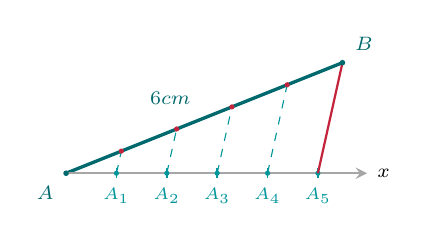
\begin{tikzpicture}[scale=0.78]
        \coordinate (A) at (0,0);
        \coordinate (B) at (4.5, 1.8);
        \draw[very thick, color=brandNavy] (A) -- (B) node[midway, above left=1pt, font=\fontsize{7}{7}\selectfont, color=brandNavy] {$6\text{cm}$};
        \draw[thick, color=gray!70, ->, >=stealth] (A) -- (4.9, 0) node[right, font=\fontsize{7.5}{7.5}\selectfont, color=black] {$x$};
        
        \foreach \i in {1,...,5} {
          \coordinate (P\i) at ({\i*0.82}, 0);
          \draw[color=brandBlue, line width=0.5pt] ($(P\i)+(0,-0.08)$) -- ($(P\i)+(0,0.08)$);
          \fill[brandBlue] (P\i) circle (1.2pt);
          \node[below=2pt, font=\fontsize{6.5}{6.5}\selectfont, color=brandBlue] at (P\i) {$A_{\i}$};
        }
        
        \draw[thick, color=brandCrimson] (P5) -- (B);
        
        \foreach \i in {1,...,4} {
          \coordinate (Q\i) at ({\i/5*4.5}, {\i/5*1.8});
          \draw[dashed, color=brandTeal] (P\i) -- (Q\i);
          \fill[brandCrimson] (Q\i) circle (1.2pt);
        }
        
        \fill[brandNavy] (A) circle (1.3pt) node[below left=1pt, font=\fontsize{7.5}{7.5}\selectfont] {$A$};
        \fill[brandNavy] (B) circle (1.3pt) node[above right=1pt, font=\fontsize{7.5}{7.5}\selectfont] {$B$};
      \end{tikzpicture}
    \end{center}
  \end{minipage}

  \vspace{3pt}
  \noindent
  \begin{minipage}{\linewidth}
    \exhead{2} ចូរចែកអង្កត់ $AB$ ដែល $AB = 8\text{cm}$ ជា $4$ ចំណែកស្មើគ្នា ។
    \begin{center}
      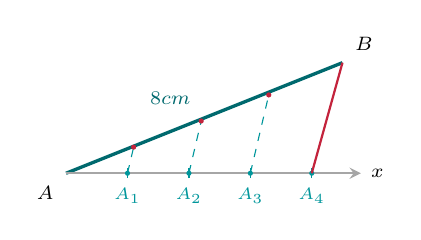
\begin{tikzpicture}[scale=0.78]
        \coordinate (A) at (0,0);
        \coordinate (B) at (4.5, 1.8);
        \draw[very thick, color=brandNavy] (A) -- (B) node[midway, above left=1pt, font=\fontsize{7}{7}\selectfont, color=brandNavy] {$8\text{cm}$};
        \draw[thick, color=gray!70, ->, >=stealth] (A) -- (4.8, 0) node[right, font=\fontsize{7.5}{7.5}\selectfont, color=black] {$x$};
        
        \foreach \i in {1,...,4} {
          \coordinate (P\i) at ({\i*1.0}, 0);
          \draw[color=brandBlue, line width=0.5pt] ($(P\i)+(0,-0.08)$) -- ($(P\i)+(0,0.08)$);
          \fill[brandBlue] (P\i) circle (1.2pt);
          \node[below=2pt, font=\fontsize{6.5}{6.5}\selectfont, color=brandBlue] at (P\i) {$A_{\i}$};
        }
        
        \draw[thick, color=brandCrimson] (P4) -- (B);
        
        \foreach \i in {1,...,3} {
          \coordinate (Q\i) at ({\i*1.1}, {\i*0.425});
          \draw[dashed, color=brandTeal] (P\i) -- (Q\i);
          \fill[brandCrimson] (Q\i) circle (1.2pt);
        }
        
        \node[below left=1pt, font=\fontsize{7.5}{7.5}\selectfont] at (A) {$A$};
        \node[above right=1pt, font=\fontsize{7.5}{7.5}\selectfont] at (B) {$B$};
      \end{tikzpicture}
    \end{center}
  \end{minipage}

  \vspace{3pt}
  \noindent
  \begin{minipage}{\linewidth}
    \exhead{3} ចូរចែកអង្កត់ $AB$ ដែល $AB = 11\text{cm}$ ជាបណ្តាអង្កត់សមាមាត្រនឹង $3, 4, 5$ ។
    \begin{center}
      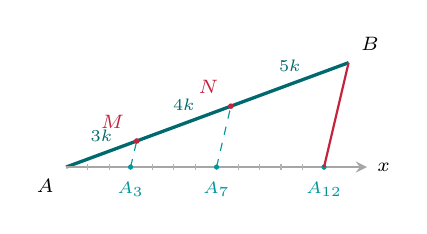
\begin{tikzpicture}[scale=0.78]
        \coordinate (A) at (0,0);
        \coordinate (B) at (4.6, 1.7);
        \coordinate (X) at (4.9, 0);
        
        \draw[very thick, color=brandNavy] (A) -- (B);
        \draw[thick, color=gray!70, ->, >=stealth] (A) -- (X) node[right, font=\fontsize{7.5}{7.5}\selectfont, color=black] {$x$};
        
        \foreach \i in {1,...,12} {
          \draw[color=gray!60, line width=0.4pt] ({\i*0.35}, -0.05) -- ({\i*0.35}, 0.05);
        }
        
        \coordinate (P3) at ({3*0.35}, 0);
        \coordinate (P7) at ({7*0.35}, 0);
        \coordinate (P12) at ({12*0.35}, 0);
        
        \fill[brandBlue] (P3) circle (1.2pt) node[below=2pt, font=\fontsize{6.5}{6.5}\selectfont, color=brandBlue] {$A_3$};
        \fill[brandBlue] (P7) circle (1.2pt) node[below=2pt, font=\fontsize{6.5}{6.5}\selectfont, color=brandBlue] {$A_7$};
        \fill[brandBlue] (P12) circle (1.2pt) node[below=2pt, font=\fontsize{6.5}{6.5}\selectfont, color=brandBlue] {$A_{12}$};
        
        \draw[thick, color=brandCrimson] (P12) -- (B);
        
        \coordinate (M) at ({3/12*4.6}, {3/12*1.7});
        \coordinate (N) at ({7/12*4.6}, {7/12*1.7});
        
        \draw[dashed, color=brandTeal] (P3) -- (M);
        \draw[dashed, color=brandTeal] (P7) -- (N);
        
        \fill[brandCrimson] (M) circle (1.3pt) node[above left=1pt, font=\fontsize{7}{7}\selectfont] {$M$};
        \fill[brandCrimson] (N) circle (1.3pt) node[above left=1pt, font=\fontsize{7}{7}\selectfont] {$N$};
        
        \node[above, font=\fontsize{6.5}{6.5}\selectfont, color=brandNavy] at ({1.5/12*4.6}, {1.5/12*1.7+0.05}) {$3k$};
        \node[above, font=\fontsize{6.5}{6.5}\selectfont, color=brandNavy] at ({5/12*4.6}, {5/12*1.7+0.05}) {$4k$};
        \node[above, font=\fontsize{6.5}{6.5}\selectfont, color=brandNavy] at ({9.5/12*4.6}, {9.5/12*1.7+0.05}) {$5k$};
        
        \node[below left=1pt, font=\fontsize{7.5}{7.5}\selectfont] at (A) {$A$};
        \node[above right=1pt, font=\fontsize{7.5}{7.5}\selectfont] at (B) {$B$};
      \end{tikzpicture}
    \end{center}
  \end{minipage}

  \columnbreak

  \noindent
  \begin{minipage}{\linewidth}
    \exhead{4} ចូរចែកអង្កត់ $AB$ ដែល $AB = 12\text{cm}$ ជាបណ្តាអង្កត់សមាមាត្រនឹង $3$, $5$, $7$ ។
    \begin{center}
      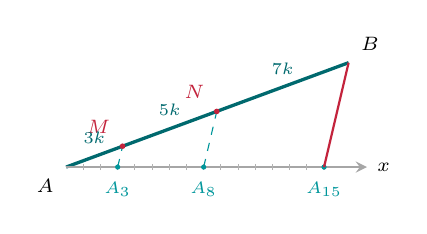
\begin{tikzpicture}[scale=0.78]
        \coordinate (A) at (0,0);
        \coordinate (B) at (4.6, 1.7);
        \coordinate (X) at (4.9, 0);
        
        \draw[very thick, color=brandNavy] (A) -- (B);
        \draw[thick, color=gray!70, ->, >=stealth] (A) -- (X) node[right, font=\fontsize{7.5}{7.5}\selectfont, color=black] {$x$};
        
        \foreach \i in {1,...,15} {
          \draw[color=gray!60, line width=0.4pt] ({\i*0.28}, -0.05) -- ({\i*0.28}, 0.05);
        }
        
        \coordinate (P3) at ({3*0.28}, 0);
        \coordinate (P8) at ({8*0.28}, 0);
        \coordinate (P15) at ({15*0.28}, 0);
        
        \fill[brandBlue] (P3) circle (1.2pt) node[below=2pt, font=\fontsize{6.5}{6.5}\selectfont, color=brandBlue] {$A_3$};
        \fill[brandBlue] (P8) circle (1.2pt) node[below=2pt, font=\fontsize{6.5}{6.5}\selectfont, color=brandBlue] {$A_8$};
        \fill[brandBlue] (P15) circle (1.2pt) node[below=2pt, font=\fontsize{6.5}{6.5}\selectfont, color=brandBlue] {$A_{15}$};
        
        \draw[thick, color=brandCrimson] (P15) -- (B);
        
        \coordinate (M) at ({3/15*4.6}, {3/15*1.7});
        \coordinate (N) at ({8/15*4.6}, {8/15*1.7});
        
        \draw[dashed, color=brandTeal] (P3) -- (M);
        \draw[dashed, color=brandTeal] (P8) -- (N);
        
        \fill[brandCrimson] (M) circle (1.3pt) node[above left=1pt, font=\fontsize{7}{7}\selectfont] {$M$};
        \fill[brandCrimson] (N) circle (1.3pt) node[above left=1pt, font=\fontsize{7}{7}\selectfont] {$N$};
        
        \node[above, font=\fontsize{6.5}{6.5}\selectfont, color=brandNavy] at ({1.5/15*4.6}, {1.5/15*1.7+0.05}) {$3k$};
        \node[above, font=\fontsize{6.5}{6.5}\selectfont, color=brandNavy] at ({5.5/15*4.6}, {5.5/15*1.7+0.05}) {$5k$};
        \node[above, font=\fontsize{6.5}{6.5}\selectfont, color=brandNavy] at ({11.5/15*4.6}, {11.5/15*1.7+0.05}) {$7k$};
        
        \node[below left=1pt, font=\fontsize{7.5}{7.5}\selectfont] at (A) {$A$};
        \node[above right=1pt, font=\fontsize{7.5}{7.5}\selectfont] at (B) {$B$};
      \end{tikzpicture}
    \end{center}
  \end{minipage}

  \vspace{3pt}
  \noindent
  \begin{minipage}{\linewidth}
    \exhead{5} គេឱ្យអង្កត់ $AB = 7\text{cm}$ ។ ចូរកំណត់ចំណុច $C$ នៅលើអង្កត់ $AB$ ដែលចែកអង្កត់ $AB$ តាមផលធៀប \koreahl{$\frac{AC}{CB} = \frac{3}{5}$} ៖
    \begin{center}
      \begin{tikzpicture}[scale=0.78]
        \coordinate (A) at (0,0);
        \coordinate (B) at (4.5, 1.7);
        \coordinate (X) at (4.8, 0);
        
        \draw[very thick, color=brandNavy] (A) -- (B);
        \draw[thick, color=gray!70, ->, >=stealth] (A) -- (X) node[right, font=\fontsize{7.5}{7.5}\selectfont, color=black] {$x$};
        
        \foreach \i in {1,...,8} {
          \coordinate (V\i) at ({\i*0.52}, 0);
          \draw[color=brandBlue, line width=0.4pt] ($(V\i)+(0,-0.08)$) -- ($(V\i)+(0,0.08)$);
        }
        \coordinate (V3) at ({3*0.52}, 0);
        \coordinate (V8) at ({8*0.52}, 0);
        \fill[brandBlue] (V3) circle (1.2pt) node[below=2pt, font=\fontsize{6.5}{6.5}\selectfont, color=brandBlue] {$A_3$};
        \fill[brandBlue] (V8) circle (1.2pt) node[below=2pt, font=\fontsize{6.5}{6.5}\selectfont, color=brandBlue] {$A_8$};
        
        \draw[thick, color=brandCrimson] (V8) -- (B);
        
        \coordinate (C) at ({3/8*4.5}, {3/8*1.7});
        \draw[dashed, color=brandTeal] (V3) -- (C);
        
        \fill[brandCrimson] (C) circle (1.3pt) node[above left=1pt, font=\fontsize{7.5}{7.5}\selectfont, color=brandCrimson] {$C$};
        \fill[brandNavy] (A) circle (1.3pt) node[below left=1pt, font=\fontsize{7.5}{7.5}\selectfont] {$A$};
        \fill[brandNavy] (B) circle (1.3pt) node[above right=1pt, font=\fontsize{7.5}{7.5}\selectfont] {$B$};
        
        \node[above, font=\fontsize{6.5}{6.5}\selectfont\kml, color=brandNavy] at ({1.5/8*4.5}, {1.5/8*1.7+0.05}) {$3$ ភាគ};
        \node[above, font=\fontsize{6.5}{6.5}\selectfont\kml, color=brandNavy] at ({5.5/8*4.5}, {5.5/8*1.7+0.05}) {$5$ ភាគ};
      \end{tikzpicture}
    \end{center}
  \end{minipage}

  \vspace{3pt}
  \noindent
  \begin{minipage}{\linewidth}
    \exhead{6} $P$ ជាចំណុចនៃអង្កត់ $AB$ ។ ចូរសង់ចំណុច $P$ ដើម្បីឱ្យបាន \koreahl{$\frac{AP}{AB} = \frac{2}{5}$} ៖
    \begin{center}
      \begin{tikzpicture}[scale=0.78]
        \coordinate (A) at (0,0);
        \coordinate (B) at (4.5, 1.6);
        \coordinate (X) at (4.8, 0);
        
        \draw[very thick, color=brandNavy] (A) -- (B);
        \draw[thick, color=gray!70, ->, >=stealth] (A) -- (X) node[right, font=\fontsize{7.5}{7.5}\selectfont, color=black] {$x$};
        
        \foreach \i in {1,...,5} {
          \coordinate (U\i) at ({\i*0.82}, 0);
          \draw[color=brandBlue, line width=0.5pt] ($(U\i)+(0,-0.08)$) -- ($(U\i)+(0,0.08)$);
          \fill[brandBlue] (U\i) circle (1.1pt);
          \node[below=2pt, font=\fontsize{6}{6}\selectfont, color=brandBlue] at (U\i) {$A_{\i}$};
        }
        
        \draw[thick, color=brandCrimson] (U5) -- (B);
        
        \coordinate (P) at ({2/5*4.5}, {2/5*1.6});
        \draw[dashed, color=brandTeal] (U2) -- (P);
        
        \fill[brandCrimson] (P) circle (1.4pt) node[above left=1pt, font=\fontsize{7.5}{7.5}\selectfont, color=brandCrimson] {$P$};
        \fill[brandNavy] (A) circle (1.4pt) node[below left=1pt, font=\fontsize{7.5}{7.5}\selectfont] {$A$};
        \fill[brandNavy] (B) circle (1.4pt) node[above right=1pt, font=\fontsize{7.5}{7.5}\selectfont] {$B$};
        
        \node[above, font=\fontsize{6.5}{6.5}\selectfont\kml, color=brandNavy] at ({1/5*4.5}, {1/5*1.6+0.06}) {$2$ ភាគ};
        \node[above, font=\fontsize{6.5}{6.5}\selectfont\kml, color=brandNavy] at ({3.5/5*4.5}, {3.5/5*1.6+0.06}) {$3$ ភាគ};
      \end{tikzpicture}
    \end{center}
  \end{minipage}
\end{multicols}

\clearpage

% =========================================================================
% PAGE 2: ផ្នែកទី ២ ៖ ទ្រឹស្ដីបទពីតាលែស
% =========================================================================
\khsection{២}{ទ្រឹស្ដីបទពីតាលែស}

\begin{khboxorange}
  \begin{minipage}[c]{0.68\textwidth}
    \begin{itemize}[leftmargin=12pt, itemsep=2.5pt, topsep=1pt, parsep=0pt]
      \item[\color{brandNavy}\ding{228}] \textbf{បើបន្ទាត់ច្រើនស្របគ្នាកាត់លើខ្នាត់ពីរកំណត់បានអង្កត់សមាមាត្រគ្នា ។}
      \item[\color{brandCrimson}\ding{228}] គេឱ្យបន្ទាត់ $AA' \parallel BB' \parallel CC'$ កាត់ខ្នាត់ $d_1$ ត្រង់ $A, B, C$ និងខ្នាត់ $d_2$ ត្រង់ $A', B', C'$ ៖
      \begin{equation*}
        \koreahl{$\frac{AB}{A'B'} = \frac{BC}{B'C'} = \frac{AC}{A'C'}$} \quad \text{ឬ} \quad \koreahl{$\frac{AB}{BC} = \frac{A'B'}{B'C'}$}
      \end{equation*}
    \end{itemize}
  \end{minipage}\hfill
  \begin{minipage}[c]{0.30\textwidth}
    \centering
    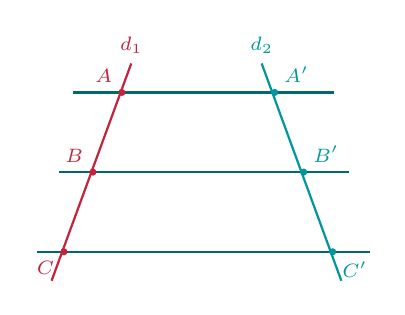
\begin{tikzpicture}[scale=0.92]
      \draw[thick, color=brandNavy] (-1.8, 2.1) -- (1.8, 2.1);
      \draw[thick, color=brandNavy] (-2.0, 1.0) -- (2.0, 1.0);
      \draw[thick, color=brandNavy] (-2.3, -0.1) -- (2.3, -0.1);
      \draw[thick, color=brandCrimson] (-1.0, 2.5) node[above, font=\fontsize{7}{7}\selectfont] {$d_1$} -- (-2.1, -0.5);
      \draw[thick, color=brandBlue] (0.8, 2.5) node[above, font=\fontsize{7}{7}\selectfont] {$d_2$} -- (1.9, -0.5);
      
      \coordinate (A) at (-1.13, 2.1);
      \coordinate (B) at (-1.53, 1.0);
      \coordinate (C) at (-1.93, -0.1);
      \coordinate (Ap) at (0.98, 2.1);
      \coordinate (Bp) at (1.38, 1.0);
      \coordinate (Cp) at (1.78, -0.1);
      
      \fill[brandCrimson] (A) circle (1.4pt) node[above left, font=\fontsize{7.5}{7.5}\selectfont] {$A$};
      \fill[brandCrimson] (B) circle (1.4pt) node[above left, font=\fontsize{7.5}{7.5}\selectfont] {$B$};
      \fill[brandCrimson] (C) circle (1.4pt) node[below left, font=\fontsize{7.5}{7.5}\selectfont] {$C$};
      
      \fill[brandBlue] (Ap) circle (1.4pt) node[above right, font=\fontsize{7.5}{7.5}\selectfont] {$A'$};
      \fill[brandBlue] (Bp) circle (1.4pt) node[above right, font=\fontsize{7.5}{7.5}\selectfont] {$B'$};
      \fill[brandBlue] (Cp) circle (1.4pt) node[below right, font=\fontsize{7.5}{7.5}\selectfont] {$C'$};
    \end{tikzpicture}
  \end{minipage}
\end{khboxorange}

\vspace{2pt}
\begin{multicols}{2}
  \noindent
  \begin{minipage}{\linewidth}
    \exhead{7} គេឱ្យបន្ទាត់ $AA' \parallel BB' \parallel CC'$ ដែលមាន $AB = 2\text{cm}$, $BC = 3\text{cm}$ និង $A'B' = 2.5\text{cm}$ ។ ចូរគណនាប្រវែង $B'C'$ ។
    \begin{center}
      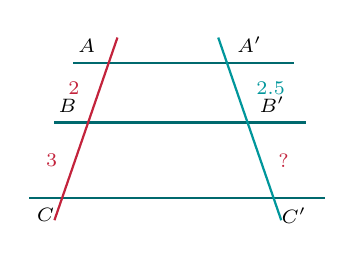
\begin{tikzpicture}[scale=0.80]
        \draw[thick, color=brandNavy] (-1.5, 1.9) -- (2.0, 1.9);
        \draw[thick, color=brandNavy] (-1.8, 0.95) -- (2.2, 0.95);
        \draw[thick, color=brandNavy] (-2.2, -0.25) -- (2.5, -0.25);
        \draw[thick, color=brandCrimson] (-0.8, 2.3) -- (-1.8, -0.6);
        \draw[thick, color=brandBlue] (0.8, 2.3) -- (1.8, -0.6);
        
        \node[above left, font=\fontsize{7}{7}\selectfont] at (-1.0, 1.9) {$A$};
        \node[above left, font=\fontsize{7}{7}\selectfont] at (-1.3, 0.95) {$B$};
        \node[below left, font=\fontsize{7}{7}\selectfont] at (-1.65, -0.25) {$C$};
        \node[above right, font=\fontsize{7}{7}\selectfont] at (0.95, 1.9) {$A'$};
        \node[above right, font=\fontsize{7}{7}\selectfont] at (1.3, 0.95) {$B'$};
        \node[below right, font=\fontsize{7}{7}\selectfont] at (1.65, -0.25) {$C'$};
        
        \node[left, font=\fontsize{7}{7}\selectfont, color=brandCrimson] at (-1.25, 1.5) {$2$};
        \node[left, font=\fontsize{7}{7}\selectfont, color=brandCrimson] at (-1.6, 0.35) {$3$};
        \node[right, font=\fontsize{7}{7}\selectfont, color=brandBlue] at (1.25, 1.5) {$2.5$};
        \node[right, font=\fontsize{7}{7}\selectfont, color=brandCrimson] at (1.6, 0.35) {$?$};
      \end{tikzpicture}
    \end{center}
  \end{minipage}

  \noindent
  \begin{minipage}{\linewidth}
    \exhead{8} គេឱ្យបន្ទាត់ $AA' \parallel BB' \parallel CC'$ ដែលមាន $AB = 6.5\text{cm}$, $B'C' = 8\text{cm}$ និង $A'B' = 3.5\text{cm}$ ។ ចូរគណនាប្រវែង $BC$ ។
    \begin{center}
      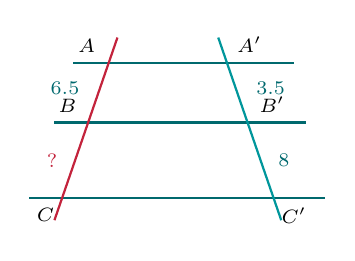
\begin{tikzpicture}[scale=0.80]
        \draw[thick, color=brandNavy] (-1.5, 1.9) -- (2.0, 1.9);
        \draw[thick, color=brandNavy] (-1.8, 0.95) -- (2.2, 0.95);
        \draw[thick, color=brandNavy] (-2.2, -0.25) -- (2.5, -0.25);
        \draw[thick, color=brandCrimson] (-0.8, 2.3) -- (-1.8, -0.6);
        \draw[thick, color=brandBlue] (0.8, 2.3) -- (1.8, -0.6);
        
        \node[above left, font=\fontsize{7}{7}\selectfont] at (-1.0, 1.9) {$A$};
        \node[above left, font=\fontsize{7}{7}\selectfont] at (-1.3, 0.95) {$B$};
        \node[below left, font=\fontsize{7}{7}\selectfont] at (-1.65, -0.25) {$C$};
        \node[above right, font=\fontsize{7}{7}\selectfont] at (0.95, 1.9) {$A'$};
        \node[above right, font=\fontsize{7}{7}\selectfont] at (1.3, 0.95) {$B'$};
        \node[below right, font=\fontsize{7}{7}\selectfont] at (1.65, -0.25) {$C'$};
        
        \node[left, font=\fontsize{7}{7}\selectfont, color=brandNavy] at (-1.25, 1.5) {$6.5$};
        \node[left, font=\fontsize{7}{7}\selectfont, color=brandCrimson] at (-1.6, 0.35) {$?$};
        \node[right, font=\fontsize{7}{7}\selectfont, color=brandNavy] at (1.25, 1.5) {$3.5$};
        \node[right, font=\fontsize{7}{7}\selectfont, color=brandNavy] at (1.6, 0.35) {$8$};
      \end{tikzpicture}
    \end{center}
  \end{minipage}

  \noindent
  \begin{minipage}{\linewidth}
    \exhead{9} គេមានបន្ទាត់ $\Delta_1$ និង $\Delta_2$ ជាបន្ទាត់ស្របគ្នា ។ តាមរូបខាងក្រោម ចូរគណនាតម្លៃនៃ $x$ គិតជា $\text{cm}$ ៖
    \begin{center}
      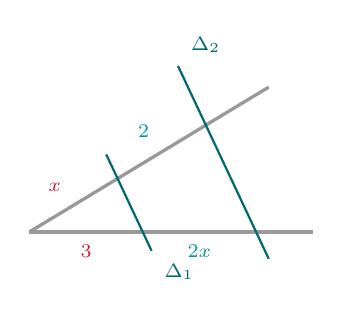
\begin{tikzpicture}[scale=0.80]
        \coordinate (O) at (0, 0);
        \coordinate (X1) at (4.5, 0);
        \coordinate (X2) at (3.8, 2.3);
        \draw[very thick, color=gray!80] (O) -- (X1);
        \draw[very thick, color=gray!80] (O) -- (X2);
        
        \coordinate (P1) at (1.8, 0);
        \coordinate (Q1) at (1.4, 0.85);
        \coordinate (P2) at (3.6, 0);
        \coordinate (Q2) at (2.8, 1.70);
        
        \draw[thick, color=brandNavy] ($(Q1)!-0.45!(P1)$) -- ($(P1)!-0.35!(Q1)$) node[at end, below right=1pt, font=\fontsize{7}{7}\selectfont, color=brandNavy] {$\Delta_1$};
        \draw[thick, color=brandNavy] ($(Q2)!-0.55!(P2)$) -- ($(P2)!-0.25!(Q2)$) node[at start, above right=1pt, font=\fontsize{7}{7}\selectfont, color=brandNavy] {$\Delta_2$};
        
        \node[above left=1pt, font=\fontsize{7}{7}\selectfont, color=brandCrimson] at (0.7, 0.45) {$x$};
        \node[above left=1pt, font=\fontsize{7}{7}\selectfont, color=brandBlue] at (2.1, 1.30) {$2$};
        \node[below=1pt, font=\fontsize{7}{7}\selectfont, color=brandCrimson] at (0.9, 0) {$3$};
        \node[below=1pt, font=\fontsize{7}{7}\selectfont, color=brandBlue] at (2.7, 0) {$2x$};
      \end{tikzpicture}
    \end{center}
  \end{minipage}

  \vspace{2pt}
  \noindent
  \begin{minipage}{\linewidth}
    \exhead{10} គេមានបន្ទាត់ស្រប $d_1 \parallel d_2 \parallel d_3$ កាត់ខ្នាត់ពីរ ។ តាមរូបខាងក្រោម ចូរគណនាតម្លៃនៃ $x$ ៖
    \begin{center}
      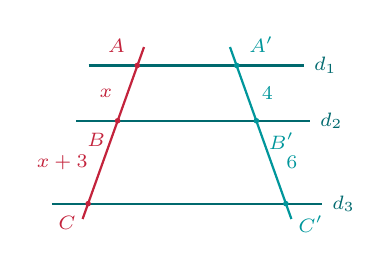
\begin{tikzpicture}[scale=0.78]
        \draw[thick, color=brandNavy] (-1.6, 1.9) -- (1.9, 1.9) node[right, font=\fontsize{7}{7}\selectfont] {$d_1$};
        \draw[thick, color=brandNavy] (-1.8, 1.0) -- (2.0, 1.0) node[right, font=\fontsize{7}{7}\selectfont] {$d_2$};
        \draw[thick, color=brandNavy] (-2.2, -0.35) -- (2.2, -0.35) node[right, font=\fontsize{7}{7}\selectfont] {$d_3$};
        
        \draw[thick, color=brandCrimson] (-0.7, 2.2) -- (-1.7, -0.6);
        \draw[thick, color=brandBlue] (0.7, 2.2) -- (1.7, -0.6);
        
        \coordinate (A) at (-0.81, 1.9);
        \coordinate (B) at (-1.13, 1.0);
        \coordinate (C) at (-1.61, -0.35);
        \coordinate (Ap) at (0.81, 1.9);
        \coordinate (Bp) at (1.13, 1.0);
        \coordinate (Cp) at (1.61, -0.35);
        
        \fill[brandCrimson] (A) circle (1.3pt) node[above left=1pt, font=\fontsize{7}{7}\selectfont] {$A$};
        \fill[brandCrimson] (B) circle (1.3pt) node[below left=1pt, font=\fontsize{7}{7}\selectfont] {$B$};
        \fill[brandCrimson] (C) circle (1.3pt) node[below left=1pt, font=\fontsize{7}{7}\selectfont] {$C$};
        
        \fill[brandBlue] (Ap) circle (1.3pt) node[above right=1pt, font=\fontsize{7}{7}\selectfont] {$A'$};
        \fill[brandBlue] (Bp) circle (1.3pt) node[below right=1pt, font=\fontsize{7}{7}\selectfont] {$B'$};
        \fill[brandBlue] (Cp) circle (1.3pt) node[below right=1pt, font=\fontsize{7}{7}\selectfont] {$C'$};
        
        \node[left=2pt, font=\fontsize{7}{7}\selectfont, color=brandCrimson] at (-0.97, 1.45) {$x$};
        \node[left=2pt, font=\fontsize{7}{7}\selectfont, color=brandCrimson] at (-1.37, 0.32) {$x+3$};
        \node[right=2pt, font=\fontsize{7}{7}\selectfont, color=brandBlue] at (0.97, 1.45) {$4$};
        \node[right=2pt, font=\fontsize{7}{7}\selectfont, color=brandBlue] at (1.37, 0.32) {$6$};
      \end{tikzpicture}
    \end{center}
  \end{minipage}

  \columnbreak

  \noindent
  \begin{minipage}{\linewidth}
    \exhead{11} គេឱ្យបន្ទាត់ $\Delta_1, \Delta_2$ និង $\Delta_3$ ជាបន្ទាត់បីស្របគ្នា ។ គេដឹងថាខ្នាត់ $d_1$ កាត់បន្ទាត់ទាំងបីត្រង់ចំណុចរៀងគ្នា $A, B$ និង $C$ ហើយខ្នាត់ $d_2$ កាត់បន្ទាត់ទាំងបីនោះត្រង់ចំណុច $D, E$ និង $F$ រៀងគ្នា ។\\
    ចូរគណនាប្រវែង $EF$ បើ $AB = 10\text{cm}$, $AC = 18.2\text{cm}$ និង $DE = 12.5\text{cm}$ ។
    \begin{center}
      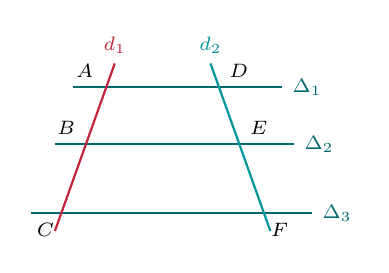
\begin{tikzpicture}[scale=0.76]
        \draw[thick, color=brandNavy] (-1.5, 1.9) -- (2.0, 1.9) node[right, font=\fontsize{7}{7}\selectfont] {$\Delta_1$};
        \draw[thick, color=brandNavy] (-1.8, 0.95) -- (2.2, 0.95) node[right, font=\fontsize{7}{7}\selectfont] {$\Delta_2$};
        \draw[thick, color=brandNavy] (-2.2, -0.2) -- (2.5, -0.2) node[right, font=\fontsize{7}{7}\selectfont] {$\Delta_3$};
        \draw[thick, color=brandCrimson] (-0.8, 2.3) node[above, font=\fontsize{7}{7}\selectfont] {$d_1$} -- (-1.8, -0.5);
        \draw[thick, color=brandBlue] (0.8, 2.3) node[above, font=\fontsize{7}{7}\selectfont] {$d_2$} -- (1.8, -0.5);
        
        \node[above left, font=\fontsize{7}{7}\selectfont] at (-1.0, 1.9) {$A$};
        \node[above left, font=\fontsize{7}{7}\selectfont] at (-1.3, 0.95) {$B$};
        \node[below left, font=\fontsize{7}{7}\selectfont] at (-1.65, -0.2) {$C$};
        \node[above right, font=\fontsize{7}{7}\selectfont] at (0.95, 1.9) {$D$};
        \node[above right, font=\fontsize{7}{7}\selectfont] at (1.3, 0.95) {$E$};
        \node[below right, font=\fontsize{7}{7}\selectfont] at (1.65, -0.2) {$F$};
      \end{tikzpicture}
    \end{center}
  \end{minipage}

  \noindent
  \begin{minipage}{\linewidth}
    \exhead{12} គេមាន $\Delta_1, \Delta_2, \Delta_3, \Delta_4$ ជាបន្ទាត់ស្របគ្នា ។ តាមរូបគំនូរខាងក្រោម ចូរគណនាតម្លៃនៃ $x$ និង $y$ ៖
    \begin{center}
      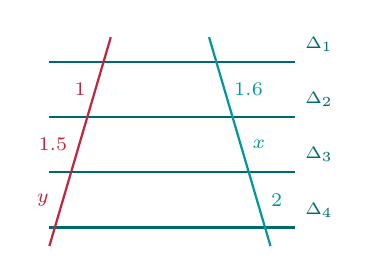
\begin{tikzpicture}[scale=0.78]
        \foreach \y/\lbl in {2.7/1, 1.8/2, 0.9/3, 0.0/4} {
          \draw[thick, color=brandNavy] (-1.8, \y) -- (2.2, \y) node[above right, font=\fontsize{6.5}{6.5}\selectfont, color=brandNavy] {$\Delta_{\lbl}$};
        }
        \draw[thick, color=brandCrimson] (-0.8, 3.1) -- (-1.8, -0.3);
        \draw[thick, color=brandBlue] (0.8, 3.1) -- (1.8, -0.3);
        
        \node[left, font=\fontsize{7}{7}\selectfont, color=brandCrimson] at (-1.05, 2.25) {$1$};
        \node[left, font=\fontsize{7}{7}\selectfont, color=brandCrimson] at (-1.35, 1.35) {$1.5$};
        \node[left, font=\fontsize{7}{7}\selectfont, color=brandCrimson] at (-1.65, 0.45) {$y$};
        
        \node[right, font=\fontsize{7}{7}\selectfont, color=brandBlue] at (1.05, 2.25) {$1.6$};
        \node[right, font=\fontsize{7}{7}\selectfont, color=brandBlue] at (1.35, 1.35) {$x$};
        \node[right, font=\fontsize{7}{7}\selectfont, color=brandBlue] at (1.65, 0.45) {$2$};
      \end{tikzpicture}
    \end{center}
  \end{minipage}

  \noindent
  \begin{minipage}{\linewidth}
    \exhead{13} គេមាន $AB \parallel CD \parallel EF \parallel GH$ តាមរូបខាងក្រោម ៖
    \begin{center}
      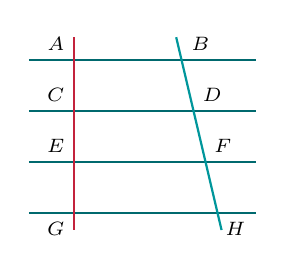
\begin{tikzpicture}[scale=0.72]
        \draw[thick, color=brandNavy] (-1.8, 2.7) -- (2.2, 2.7);
        \draw[thick, color=brandNavy] (-1.8, 1.8) -- (2.2, 1.8);
        \draw[thick, color=brandNavy] (-1.8, 0.9) -- (2.2, 0.9);
        \draw[thick, color=brandNavy] (-1.8, 0.0) -- (2.2, 0.0);
        
        \draw[thick, color=brandCrimson] (-1.0, 3.1) -- (-1.0, -0.3);
        \draw[thick, color=brandBlue] (0.8, 3.1) -- (1.6, -0.3);
        
        \node[above left, font=\fontsize{7}{7}\selectfont] at (-1.0, 2.7) {$A$};
        \node[above left, font=\fontsize{7}{7}\selectfont] at (-1.0, 1.8) {$C$};
        \node[above left, font=\fontsize{7}{7}\selectfont] at (-1.0, 0.9) {$E$};
        \node[below left, font=\fontsize{7}{7}\selectfont] at (-1.0, 0.0) {$G$};
        
        \node[above right, font=\fontsize{7}{7}\selectfont] at (0.9, 2.7) {$B$};
        \node[above right, font=\fontsize{7}{7}\selectfont] at (1.1, 1.8) {$D$};
        \node[above right, font=\fontsize{7}{7}\selectfont] at (1.3, 0.9) {$F$};
        \node[below right, font=\fontsize{7}{7}\selectfont] at (1.5, 0.0) {$H$};
      \end{tikzpicture}
    \end{center}
    \begin{itemize}[leftmargin=12pt, itemsep=1.5pt, topsep=1pt, parsep=0pt]
      \item[\khlabel{ក}] គណនា $DF$ និង $FH$ បើ $AC = 6\text{cm}$, $CE = 12\text{cm}$, $EG = 4\text{cm}$ និង $BD = 9\text{cm}$ ។
      \item[\khlabel{ខ}] គណនា $BD, DF$ និង $FH$ បើ $AC = 6\text{cm}$, $CE = 12\text{cm}$, $EG = 4\text{cm}$ និង $HB = 33\text{cm}$ ។
      \item[\khlabel{គ}] គណនា $DF$ និង $CG$ បើ $AC = 6\text{cm}$, $CE = 12\text{cm}$, $DB = 8\text{cm}$ និង $FH = 6\text{cm}$ ។
    \end{itemize}
  \end{minipage}
\end{multicols}

\clearpage

% =========================================================================
% PAGE 3: ផ្នែកទី ៣ ៖ អនុវត្តន៍ក្នុងត្រីកោណ
% =========================================================================
\khsection{៣}{អនុវត្តន៍ក្នុងត្រីកោណ និងចតុកោណព្នាយ}

\khsubsection{៣.១}{អនុវត្តន៍ក្នុងត្រីកោណ}

\begin{khboxorange}
  \begin{minipage}[c]{0.68\textwidth}
    \begin{itemize}[leftmargin=12pt, itemsep=2.5pt, topsep=1pt, parsep=0pt]
      \item[\color{brandNavy}\ding{228}] \textbf{ទ្រឹស្ដីបទតាលែសក្នុងត្រីកោណ ៖} $EF$ ជាបន្ទាត់កាត់ជ្រុងពីរនៃត្រីកោណ $ABC$ ៖
      \begin{equation*}
        \text{បើ } EF \parallel BC \implies \koreahl{$\frac{AE}{AB} = \frac{AF}{AC} = \frac{EF}{BC}$} \quad \left(\text{ឬ } \frac{AE}{EB} = \frac{AF}{FC}\right)
      \end{equation*}
      \item[\color{brandCrimson}\ding{228}] \textbf{ទ្រឹស្ដីបទច្រាស ៖} បើ $\displaystyle\frac{AE}{AB} = \frac{AF}{AC}$ (ឬ $\frac{AE}{EB} = \frac{AF}{FC}$) នោះគេបាន \koreahl{$EF \parallel BC$}
      \item[\color{brandNavy}\ding{228}] \textbf{ការស្រាយបញ្ជាក់ ៖} គូស $EN \parallel AC$ ($N \in BC$) នោះ $ENFC$ ជាប្រលេឡូក្រាម $\implies NC = EF$ និង $\frac{EF}{BC} = \frac{AE}{AB}$ ។ ដូចនេះ $\frac{AE}{AB} = \frac{AF}{AC} = \frac{EF}{BC}$ (ពិត) ។
    \end{itemize}
  \end{minipage}\hfill
  \begin{minipage}[c]{0.30\textwidth}
    \centering
    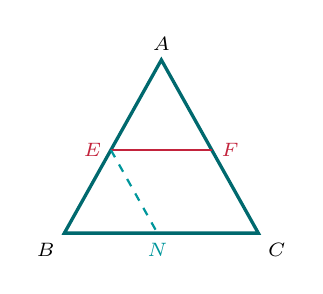
\begin{tikzpicture}[scale=0.88]
      \coordinate (A) at (1.4, 2.5);
      \coordinate (B) at (0.0, 0.0);
      \coordinate (C) at (2.8, 0.0);
      \coordinate (E) at ($(A)!0.52!(B)$);
      \coordinate (F) at ($(A)!0.52!(C)$);
      \coordinate (N) at ($(B)!0.48!(C)$);
      
      \draw[very thick, color=brandNavy] (A) -- (B) -- (C) -- cycle;
      \draw[thick, color=brandCrimson] (E) -- (F);
      \draw[thick, dashed, color=brandBlue] (E) -- (N);
      
      \node[above, font=\fontsize{7.5}{7.5}\selectfont] at (A) {$A$};
      \node[below left, font=\fontsize{7.5}{7.5}\selectfont] at (B) {$B$};
      \node[below right, font=\fontsize{7.5}{7.5}\selectfont] at (C) {$C$};
      \node[left, font=\fontsize{7.5}{7.5}\selectfont, color=brandCrimson] at (E) {$E$};
      \node[right, font=\fontsize{7.5}{7.5}\selectfont, color=brandCrimson] at (F) {$F$};
      \node[below, font=\fontsize{7.5}{7.5}\selectfont, color=brandBlue] at (N) {$N$};
    \end{tikzpicture}
  \end{minipage}
\end{khboxorange}

\vspace{2pt}
\noindent
\exhead{14} គេឱ្យបន្ទាត់ $(AB) \parallel (MN)$ ។ ចូរគណនាប្រវែង $x$ ក្នុងរូបនីមួយៗខាងក្រោម ៖
\begin{center}
  \begin{tikzpicture}[scale=0.88]
    % Figure 1 (ក)
    \begin{scope}[xshift=0cm]
      \coordinate (A) at (1.3, 2.1);
      \coordinate (B) at (0, 0);
      \coordinate (C) at (2.6, 0);
      \coordinate (M) at ($(A)!0.4!(B)$);
      \coordinate (N) at ($(A)!0.4!(C)$);
      
      \draw[very thick, color=brandNavy] (A) -- (B) -- (C) -- cycle;
      \draw[thick, color=brandCrimson] (M) -- (N);
      
      \node[above, font=\fontsize{7.5}{7.5}\selectfont] at (A) {$A$};
      \node[below left, font=\fontsize{7.5}{7.5}\selectfont] at (B) {$B$};
      \node[below right, font=\fontsize{7.5}{7.5}\selectfont] at (C) {$C$};
      \node[left, font=\fontsize{7.5}{7.5}\selectfont, color=brandCrimson] at (M) {$M$};
      \node[right, font=\fontsize{7.5}{7.5}\selectfont, color=brandCrimson] at (N) {$N$};
      
      \node[left, font=\fontsize{7}{7}\selectfont, color=brandNavy] at ($(A)!0.5!(M)$) {$9$};
      \node[left, font=\fontsize{7}{7}\selectfont, color=brandNavy] at ($(M)!0.5!(B)$) {$16$};
      \node[right, font=\fontsize{7}{7}\selectfont, color=brandNavy] at ($(A)!0.5!(N)$) {$8$};
      \node[right, font=\fontsize{7}{7}\selectfont, color=brandCrimson] at ($(N)!0.5!(C)$) {$x$};
      \node[below, font=\fontsize{7.5}{7.5}\selectfont] at (1.3, -0.3) {\khlabel{ក}};
    \end{scope}

    % Figure 2 (ខ)
    \begin{scope}[xshift=6.5cm]
      \coordinate (A) at (1.3, 2.1);
      \coordinate (B) at (0, 0);
      \coordinate (C) at (2.6, 0);
      \coordinate (M) at ($(A)!0.6!(B)$);
      \coordinate (N) at ($(A)!0.6!(C)$);
      
      \draw[very thick, color=brandNavy] (A) -- (B) -- (C) -- cycle;
      \draw[thick, color=brandCrimson] (M) -- (N);
      
      \node[above, font=\fontsize{7.5}{7.5}\selectfont] at (A) {$A$};
      \node[below left, font=\fontsize{7.5}{7.5}\selectfont] at (B) {$B$};
      \node[below right, font=\fontsize{7.5}{7.5}\selectfont] at (C) {$C$};
      \node[left, font=\fontsize{7.5}{7.5}\selectfont, color=brandCrimson] at (M) {$M$};
      \node[right, font=\fontsize{7.5}{7.5}\selectfont, color=brandCrimson] at (N) {$N$};
      
      \node[left, font=\fontsize{7}{7}\selectfont, color=brandNavy] at ($(A)!0.5!(M)$) {$8$};
      \node[left, font=\fontsize{7}{7}\selectfont, color=brandNavy] at ($(M)!0.5!(B)$) {$3$};
      \node[right, font=\fontsize{7}{7}\selectfont, color=brandCrimson] at ($(A)!0.5!(N)$) {$x$};
      \node[right, font=\fontsize{7}{7}\selectfont, color=brandNavy] at ($(N)!0.5!(C)$) {$4$};
      \node[below, font=\fontsize{7.5}{7.5}\selectfont] at (1.3, -0.3) {\khlabel{ខ}};
    \end{scope}

    % Figure 3 (គ)
    \begin{scope}[xshift=13cm]
      \coordinate (A) at (0.8, 2.1);
      \coordinate (B) at (0, 0);
      \coordinate (C) at (3.0, 0);
      \coordinate (M) at ($(A)!0.45!(C)$);
      \coordinate (N) at ($(B)!0.3!(C)$);
      
      \draw[very thick, color=brandNavy] (A) -- (B) -- (C) -- cycle;
      \draw[thick, color=brandCrimson] (M) -- (N);
      
      \node[above, font=\fontsize{7.5}{7.5}\selectfont] at (A) {$A$};
      \node[below left, font=\fontsize{7.5}{7.5}\selectfont] at (B) {$B$};
      \node[below right, font=\fontsize{7.5}{7.5}\selectfont] at (C) {$C$};
      \node[above right, font=\fontsize{7.5}{7.5}\selectfont, color=brandCrimson] at (M) {$M$};
      \node[below, font=\fontsize{7.5}{7.5}\selectfont, color=brandCrimson] at (N) {$N$};
      
      \node[above right, font=\fontsize{7}{7}\selectfont, color=brandCrimson] at ($(A)!0.5!(M)$) {$x$};
      \node[above right, font=\fontsize{7}{7}\selectfont, color=brandNavy] at ($(M)!0.5!(C)$) {$6$};
      \node[below, font=\fontsize{7}{7}\selectfont, color=brandNavy] at ($(B)!0.5!(N)$) {$4$};
      \draw[<->, >=stealth, color=brandNavy, line width=0.4pt] (0, -0.4) -- (3.0, -0.4) node[midway, fill=white, inner sep=1pt, font=\fontsize{6.5}{6.5}\selectfont] {$12$};
      \node[below, font=\fontsize{7.5}{7.5}\selectfont] at (1.5, -0.65) {\khlabel{គ}};
    \end{scope}
  \end{tikzpicture}
\end{center}

\vspace{1pt}
\noindent
\exhead{15} ចូរគណនាប្រវែង $a$ និង $b$ គិតជា $\text{cm}$ តាមរូបនីមួយៗខាងក្រោម ៖
\begin{center}
  \begin{tikzpicture}[scale=0.88]
    % Figure 1 (ក)
    \begin{scope}[xshift=0cm]
      \coordinate (C) at (1.4, 2.1);
      \coordinate (A) at (0, 0);
      \coordinate (B) at (2.8, 0);
      \coordinate (E) at ($(C)!0.4!(A)$);
      \coordinate (F) at ($(C)!0.4!(B)$);
      
      \draw[very thick, color=brandNavy] (C) -- (A) -- (B) -- cycle;
      \draw[thick, color=brandCrimson] (E) -- (F);
      
      \node[above, font=\fontsize{7.5}{7.5}\selectfont] at (C) {$C$};
      \node[below left, font=\fontsize{7.5}{7.5}\selectfont] at (A) {$A$};
      \node[below right, font=\fontsize{7.5}{7.5}\selectfont] at (B) {$B$};
      \node[left, font=\fontsize{7.5}{7.5}\selectfont, color=brandCrimson] at (E) {$E$};
      \node[right, font=\fontsize{7.5}{7.5}\selectfont, color=brandCrimson] at (F) {$F$};
      
      \node[left, font=\fontsize{7}{7}\selectfont, color=brandCrimson] at ($(C)!0.5!(E)$) {$a$};
      \node[left, font=\fontsize{7}{7}\selectfont, color=brandNavy] at ($(E)!0.5!(A)$) {$20$};
      \node[right, font=\fontsize{7}{7}\selectfont, color=brandNavy] at ($(C)!0.5!(F)$) {$8$};
      \node[right, font=\fontsize{7}{7}\selectfont, color=brandNavy] at ($(F)!0.5!(B)$) {$18$};
      \node[above, font=\fontsize{7}{7}\selectfont, color=brandCrimson] at ($(E)!0.5!(F)$) {$b$};
      \node[below, font=\fontsize{7}{7}\selectfont, color=brandNavy] at ($(A)!0.5!(B)$) {$25$};
      \node[below, font=\fontsize{7.5}{7.5}\selectfont] at (1.4, -0.35) {\khlabel{ក} $EF \parallel AB$};
    \end{scope}

    % Figure 2 (ខ)
    \begin{scope}[xshift=6.5cm]
      \coordinate (M) at (1.4, 2.1);
      \coordinate (N) at (0, 0);
      \coordinate (P) at (2.8, 0);
      \coordinate (A) at ($(M)!0.55!(N)$);
      \coordinate (B) at ($(M)!0.55!(P)$);
      
      \draw[very thick, color=brandNavy] (M) -- (N) -- (P) -- cycle;
      \draw[thick, color=brandCrimson] (A) -- (B);
      
      \node[above, font=\fontsize{7.5}{7.5}\selectfont] at (M) {$M$};
      \node[below left, font=\fontsize{7.5}{7.5}\selectfont] at (N) {$N$};
      \node[below right, font=\fontsize{7.5}{7.5}\selectfont] at (P) {$P$};
      \node[left, font=\fontsize{7.5}{7.5}\selectfont, color=brandCrimson] at (A) {$A$};
      \node[right, font=\fontsize{7.5}{7.5}\selectfont, color=brandCrimson] at (B) {$B$};
      
      \node[left, font=\fontsize{7}{7}\selectfont, color=brandNavy] at ($(M)!0.5!(A)$) {$25$};
      \node[left, font=\fontsize{7}{7}\selectfont, color=brandCrimson] at ($(A)!0.5!(N)$) {$3a$};
      \node[right, font=\fontsize{7}{7}\selectfont, color=brandNavy] at ($(M)!0.5!(B)$) {$20$};
      \node[right, font=\fontsize{7}{7}\selectfont, color=brandNavy] at ($(B)!0.5!(P)$) {$12.4$};
      \node[above, font=\fontsize{7}{7}\selectfont, color=brandNavy] at ($(A)!0.5!(B)$) {$b$};
      \node[below, font=\fontsize{7.5}{7.5}\selectfont, color=brandNavy] at ($(N)!0.5!(P)$) {$42.5$};
      \node[below, font=\fontsize{7.5}{7.5}\selectfont] at (1.4, -0.35) {\khlabel{ខ} $AB \parallel NP$};
    \end{scope}

    % Figure 3 (គ)
    \begin{scope}[xshift=13cm]
      \coordinate (A) at (0.7, 2.1);
      \coordinate (B) at (0, 0);
      \coordinate (C) at (3.1, 0);
      \coordinate (M) at ($(A)!0.45!(C)$);
      \coordinate (N) at ($(B)!0.28!(C)$);
      
      \draw[very thick, color=brandNavy] (A) -- (B) -- (C) -- cycle;
      \draw[thick, color=brandCrimson] (M) -- (N);
      
      \node[above, font=\fontsize{7.5}{7.5}\selectfont] at (A) {$A$};
      \node[below left, font=\fontsize{7.5}{7.5}\selectfont] at (B) {$B$};
      \node[below right, font=\fontsize{7.5}{7.5}\selectfont] at (C) {$C$};
      \node[above right, font=\fontsize{7.5}{7.5}\selectfont, color=brandCrimson] at (M) {$M$};
      \node[below, font=\fontsize{7.5}{7.5}\selectfont, color=brandCrimson] at (N) {$N$};
      
      \node[left, font=\fontsize{7}{7}\selectfont, color=brandNavy] at ($(A)!0.5!(B)$) {$12$};
      \node[above right, font=\fontsize{7}{7}\selectfont, color=brandNavy] at ($(M)!0.5!(C)$) {$6$};
      \node[above, font=\fontsize{7}{7}\selectfont, color=brandCrimson] at ($(M)!0.5!(N)$) {$a$};
      \node[below, font=\fontsize{7.5}{7.5}\selectfont, color=brandNavy] at ($(B)!0.5!(N)$) {$4.2$};
      \draw[<->, >=stealth, color=brandCrimson, line width=0.4pt] (0, -0.35) -- (3.1, -0.35) node[midway, fill=white, inner sep=1pt, font=\fontsize{6.5}{6.5}\selectfont] {$b$};
      
      \node[below, font=\fontsize{7.5}{7.5}\selectfont] at (1.55, -0.65) {\khlabel{គ} $MN \parallel AB$};
    \end{scope}
  \end{tikzpicture}
\end{center}

\vspace{1pt}
\begin{multicols}{2}
  \noindent
  \begin{minipage}{\linewidth}
    \exhead{16} ក្នុងត្រីកោណមួយមាន $AB \parallel DC$ ។ ចូរគណនាតម្លៃនៃ $x$ គិតជា $\text{cm}$ ៖
    \begin{center}
      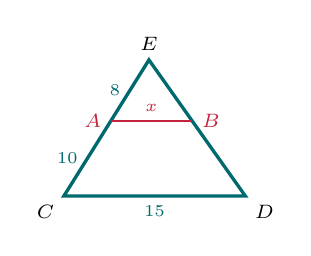
\begin{tikzpicture}[scale=0.72]
        \coordinate (E) at (1.5, 2.4);
        \coordinate (C) at (0.0, 0.0);
        \coordinate (D) at (3.2, 0.0);
        \coordinate (A) at ($(E)!0.45!(C)$);
        \coordinate (B) at ($(E)!0.45!(D)$);
        
        \draw[very thick, color=brandNavy] (E) -- (C) -- (D) -- cycle;
        \draw[thick, color=brandCrimson] (A) -- (B);
        
        \node[above, font=\fontsize{7}{7}\selectfont] at (E) {$E$};
        \node[below left, font=\fontsize{7}{7}\selectfont] at (C) {$C$};
        \node[below right, font=\fontsize{7}{7}\selectfont] at (D) {$D$};
        \node[left, font=\fontsize{7}{7}\selectfont, color=brandCrimson] at (A) {$A$};
        \node[right, font=\fontsize{7}{7}\selectfont, color=brandCrimson] at (B) {$B$};
        
        \node[left, font=\fontsize{6.5}{6.5}\selectfont, color=brandNavy] at ($(E)!0.5!(A)$) {$8$};
        \node[left, font=\fontsize{6.5}{6.5}\selectfont, color=brandNavy] at ($(A)!0.5!(C)$) {$10$};
        \node[above, font=\fontsize{6.5}{6.5}\selectfont, color=brandCrimson] at ($(A)!0.5!(B)$) {$x$};
        \node[below, font=\fontsize{6.5}{6.5}\selectfont, color=brandNavy] at ($(C)!0.5!(D)$) {$15$};
      \end{tikzpicture}
    \end{center}
  \end{minipage}

  \noindent
  \begin{minipage}{\linewidth}
    \exhead{17} ក្នុងត្រីកោណ $PTQ$ គេមានចំណុច $N \in PQ$ និង $R \in PT$ ដែល $PN = 6$, $PR = 12$, $RT = 4$ និង $NQ = 2$ ។\\
    ចូរស្រាយបញ្ជាក់ថា \koreahl{$NR \parallel QT$} ។
    \begin{center}
      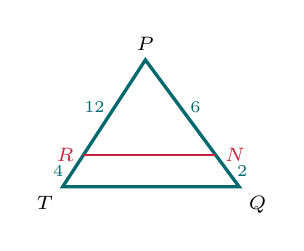
\begin{tikzpicture}[scale=0.70]
        \coordinate (P) at (1.5, 2.3);
        \coordinate (T) at (0, 0);
        \coordinate (Q) at (3.2, 0);
        \coordinate (R) at ($(P)!0.75!(T)$);
        \coordinate (N) at ($(P)!0.75!(Q)$);
        
        \draw[very thick, color=brandNavy] (P) -- (T) -- (Q) -- cycle;
        \draw[thick, color=brandCrimson] (R) -- (N);
        
        \node[above, font=\fontsize{7}{7}\selectfont] at (P) {$P$};
        \node[below left, font=\fontsize{7}{7}\selectfont] at (T) {$T$};
        \node[below right, font=\fontsize{7}{7}\selectfont] at (Q) {$Q$};
        \node[left, font=\fontsize{7}{7}\selectfont, color=brandCrimson] at (R) {$R$};
        \node[right, font=\fontsize{7}{7}\selectfont, color=brandCrimson] at (N) {$N$};
        
        \node[left, font=\fontsize{6.5}{6.5}\selectfont, color=brandNavy] at ($(P)!0.5!(R)$) {$12$};
        \node[left, font=\fontsize{6.5}{6.5}\selectfont, color=brandNavy] at ($(R)!0.5!(T)$) {$4$};
        \node[right, font=\fontsize{6.5}{6.5}\selectfont, color=brandNavy] at ($(P)!0.5!(N)$) {$6$};
        \node[right, font=\fontsize{6.5}{6.5}\selectfont, color=brandNavy] at ($(N)!0.5!(Q)$) {$2$};
      \end{tikzpicture}
    \end{center}
  \end{minipage}

  \columnbreak

  \noindent
  \begin{minipage}{\linewidth}
    \exhead{18} តាមរូបខាងក្រោម គេមានបន្ទាត់ $BE \parallel CD$ ។ ចូរគណនាប្រវែង $ED$ និង $CD$ ដោយដឹងថារង្វាស់គិតជា $\text{cm}$ ៖
    \begin{center}
      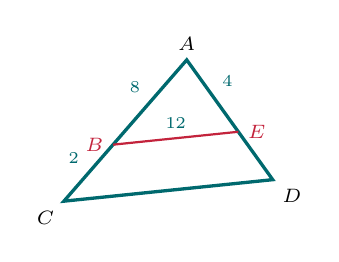
\begin{tikzpicture}[scale=0.78]
        \coordinate (A) at (2.0, 2.3);
        \coordinate (C) at (0.0, 0.0);
        \coordinate (D) at (3.4, 0.35);
        \coordinate (B) at ($(A)!0.6!(C)$);
        \coordinate (E) at ($(A)!0.6!(D)$);
        
        \draw[very thick, color=brandNavy] (A) -- (C) -- (D) -- cycle;
        \draw[thick, color=brandCrimson] (B) -- (E);
        
        \node[above, font=\fontsize{7}{7}\selectfont] at (A) {$A$};
        \node[below left, font=\fontsize{7}{7}\selectfont] at (C) {$C$};
        \node[below right, font=\fontsize{7}{7}\selectfont] at (D) {$D$};
        \node[left, font=\fontsize{7}{7}\selectfont, color=brandCrimson] at (B) {$B$};
        \node[right, font=\fontsize{7}{7}\selectfont, color=brandCrimson] at (E) {$E$};
        
        \node[above left, font=\fontsize{6.5}{6.5}\selectfont, color=brandNavy] at ($(A)!0.5!(B)$) {$8$};
        \node[above left, font=\fontsize{6.5}{6.5}\selectfont, color=brandNavy] at ($(B)!0.5!(C)$) {$2$};
        \node[above right, font=\fontsize{6.5}{6.5}\selectfont, color=brandNavy] at ($(A)!0.5!(E)$) {$4$};
        \node[above, font=\fontsize{6.5}{6.5}\selectfont, color=brandNavy] at ($(B)!0.5!(E)$) {$12$};
      \end{tikzpicture}
    \end{center}
  \end{minipage}

  \noindent
  \begin{minipage}{\linewidth}
    \exhead{19} ចូរគណនាប្រវែង $a$ និង $b$ តាមរូបខាងក្រោមនេះ ដោយដឹងថារង្វាស់គិតជា $\text{cm}$ ៖
    \begin{center}
      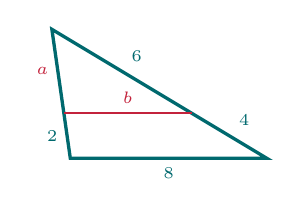
\begin{tikzpicture}[scale=0.78]
        \coordinate (P) at (0, 2.1);
        \coordinate (Q) at (0.3, 0);
        \coordinate (R) at (3.5, 0);
        \coordinate (M) at ($(P)!0.65!(Q)$);
        \coordinate (N) at ($(P)!0.65!(R)$);
        
        \draw[very thick, color=brandNavy] (P) -- (Q) -- (R) -- cycle;
        \draw[thick, color=brandCrimson] (M) -- (N);
        
        \node[left, font=\fontsize{6.5}{6.5}\selectfont, color=brandCrimson] at ($(P)!0.5!(M)$) {$a$};
        \node[left, font=\fontsize{6.5}{6.5}\selectfont, color=brandNavy] at ($(M)!0.5!(Q)$) {$2$};
        \node[above, font=\fontsize{6.5}{6.5}\selectfont, color=brandCrimson] at ($(M)!0.5!(N)$) {$b$};
        \node[above right, font=\fontsize{6.5}{6.5}\selectfont, color=brandNavy] at ($(P)!0.5!(N)$) {$6$};
        \node[above right, font=\fontsize{6.5}{6.5}\selectfont, color=brandNavy] at ($(N)!0.5!(R)$) {$4$};
        \node[below, font=\fontsize{6.5}{6.5}\selectfont, color=brandNavy] at ($(Q)!0.5!(R)$) {$8$};
      \end{tikzpicture}
    \end{center}
  \end{minipage}
\end{multicols}

\clearpage

% =========================================================================
% PAGE 4: ចំណោទដើមឈើ & ៣.២ អនុវត្តន៍ក្នុងចតុកោណព្នាយ
% =========================================================================
\begin{multicols}{2}
  \noindent
  \begin{minipage}{\linewidth}
    \exhead{20} {\bfseries ចំណោទអនុវត្តន៍វាស់កម្ពស់ដើមឈើ ៖}\\
    គេចង់វាស់កម្ពស់ដើមឈើមួយដើម ។ គេយកបង្គោលមួយដើមមកដាក់ក្នុងម្លប់ដើមឈើនោះ ហើយគេរំកិលវាដោយលៃឱ្យស្រមោលនៃចុងបង្គោល $E$ និងស្រមោលនៃចុងឈើ $A$ ត្រួតស៊ីគ្នាត្រង់ចំណុច $C$ ។\\
    ដោយស្គាល់ប្រវែងបង្គោល $DE = 1.08\text{m}$ ប្រវែងស្រមោលបង្គោល $CD = 0.9\text{m}$ និងប្រវែងស្រមោលដើមឈើ $CB = 12.45\text{m}$ ។ ចូររកកម្ពស់ដើមឈើនោះ ។
    \begin{center}
      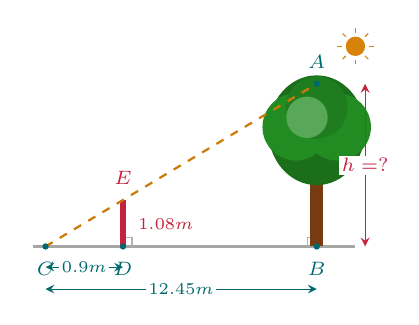
\begin{tikzpicture}[scale=0.82]
        \coordinate (C) at (0, 0);
        \coordinate (B) at (4.2, 0);
        \coordinate (A) at (4.2, 2.52);
        \coordinate (D) at (1.2, 0);
        \coordinate (E) at (1.2, 0.72);
        
        % Ground line
        \draw[very thick, color=gray!70] (-0.2, 0) -- (4.8, 0);
        
        % Right angle markers
        \draw[color=gray!60, line width=0.4pt] (1.2, 0.14) -- (1.34, 0.14) -- (1.34, 0);
        \draw[color=gray!60, line width=0.4pt] (4.06, 0) -- (4.06, 0.14) -- (4.2, 0.14);
        
        % Pole at D
        \draw[line width=2.2pt, color=brandCrimson] (D) -- (E);
        \node[above=2pt, font=\fontsize{7}{7}\selectfont, color=brandCrimson] at (E) {$E$};
        \node[right=2pt, font=\fontsize{6.5}{6.5}\selectfont, color=brandCrimson] at (1.2, 0.34) {$1.08\text{m}$};
        
        % Stylized tree at B
        \draw[line width=4.5pt, color=treeBrown!85!black] (4.2, 0) -- (4.2, 1.3);
        \fill[treeGreen!80!black] (4.2, 1.8) ellipse (0.75 and 0.85);
        \fill[treeGreen] (3.88, 1.85) circle (0.52);
        \fill[treeGreen] (4.52, 1.85) circle (0.52);
        \fill[treeGreen!90!black] (4.2, 2.15) circle (0.48);
        \fill[treeGreen!75!white] (4.05, 2.0) circle (0.32);
        
        % Sun ray
        \draw[thick, dashed, color=brandGold!95!black] (C) -- (A);
        
        % Mini sun
        \fill[brandGold] (4.8, 3.1) circle (0.15);
        \foreach \a in {0, 45, ..., 315} {
          \draw[line width=0.4pt, color=brandGold] ({4.8 + 0.21*cos(\a)}, {3.1 + 0.21*sin(\a)}) -- ({4.8 + 0.28*cos(\a)}, {3.1 + 0.28*sin(\a)});
        }
        
        % Points & labels
        \fill[brandNavy] (C) circle (1.4pt) node[below=2pt, font=\fontsize{7.5}{7.5}\selectfont] {$C$};
        \fill[brandNavy] (D) circle (1.4pt) node[below=2pt, font=\fontsize{7.5}{7.5}\selectfont] {$D$};
        \fill[brandNavy] (B) circle (1.4pt) node[below=2pt, font=\fontsize{7.5}{7.5}\selectfont] {$B$};
        \fill[brandNavy] (A) circle (1.4pt) node[above=2pt, font=\fontsize{7.5}{7.5}\selectfont] {$A$};
        
        % Dimension lines
        \draw[<->, >=stealth, color=brandNavy, line width=0.4pt] (0, -0.32) -- (1.2, -0.32) node[midway, fill=white, inner sep=1pt, font=\fontsize{6.5}{6.5}\selectfont] {$0.9\text{m}$};
        \draw[<->, >=stealth, color=brandNavy, line width=0.4pt] (0, -0.66) -- (4.2, -0.66) node[midway, fill=white, inner sep=1pt, font=\fontsize{6.5}{6.5}\selectfont] {$12.45\text{m}$};
        \draw[<->, >=stealth, color=brandCrimson, line width=0.45pt] (4.95, 0) -- (4.95, 2.52) node[midway, fill=white, inner sep=1pt, font=\fontsize{7}{7}\selectfont] {$h = ?$};
      \end{tikzpicture}
    \end{center}
  \end{minipage}

  \columnbreak

  \noindent
  \begin{minipage}{\linewidth}
    \exhead{21} គ្រូនាំសិស្សចេញក្រៅថ្នាក់ដើម្បីអនុវត្តន៍វាស់កម្ពស់ដើមឈើមួយដើមដែលស្ថិតនៅក្នុងទីធ្លាសាលា ។ ដោយឱ្យសិស្សម្នាក់យកបង្គោលមួយដើមដែលមានប្រវែង $1\text{m}$ មកដាក់ក្នុងម្លប់ដើមឈើនោះ ហើយរំកិលឱ្យស្រមោលនៃចុងបង្គោល និងស្រមោលនៃចុងឈើត្រួតស៊ីគ្នា ។\\
    ប្រសិនបើវាស់ដឹងថា ស្រមោលបង្គោលមានប្រវែង $1.2\text{m}$ និងស្រមោលដើមឈើមានប្រវែង $15.6\text{m}$ ចូរគណនាកម្ពស់នៃដើមឈើនោះ ។
    \begin{center}
      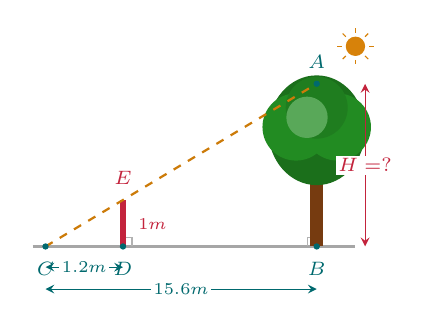
\begin{tikzpicture}[scale=0.82]
        \coordinate (C) at (0, 0);
        \coordinate (B) at (4.2, 0);
        \coordinate (A) at (4.2, 2.52);
        \coordinate (D) at (1.2, 0);
        \coordinate (E) at (1.2, 0.72);
        
        % Ground line
        \draw[very thick, color=gray!70] (-0.2, 0) -- (4.8, 0);
        
        % Right angle markers
        \draw[color=gray!60, line width=0.4pt] (1.2, 0.14) -- (1.34, 0.14) -- (1.34, 0);
        \draw[color=gray!60, line width=0.4pt] (4.06, 0) -- (4.06, 0.14) -- (4.2, 0.14);
        
        % Pole at D
        \draw[line width=2.2pt, color=brandCrimson] (D) -- (E);
        \node[above=2pt, font=\fontsize{7}{7}\selectfont, color=brandCrimson] at (E) {$E$};
        \node[right=2pt, font=\fontsize{6.5}{6.5}\selectfont, color=brandCrimson] at (1.2, 0.34) {$1\text{m}$};
        
        % Stylized tree at B
        \draw[line width=4.5pt, color=treeBrown!85!black] (4.2, 0) -- (4.2, 1.3);
        \fill[treeGreen!80!black] (4.2, 1.8) ellipse (0.75 and 0.85);
        \fill[treeGreen] (3.88, 1.85) circle (0.52);
        \fill[treeGreen] (4.52, 1.85) circle (0.52);
        \fill[treeGreen!90!black] (4.2, 2.15) circle (0.48);
        \fill[treeGreen!75!white] (4.05, 2.0) circle (0.32);
        
        % Sun ray
        \draw[thick, dashed, color=brandGold!95!black] (C) -- (A);
        
        % Mini sun
        \fill[brandGold] (4.8, 3.1) circle (0.15);
        \foreach \a in {0, 45, ..., 315} {
          \draw[line width=0.4pt, color=brandGold] ({4.8 + 0.21*cos(\a)}, {3.1 + 0.21*sin(\a)}) -- ({4.8 + 0.28*cos(\a)}, {3.1 + 0.28*sin(\a)});
        }
        
        % Points & labels
        \fill[brandNavy] (C) circle (1.4pt) node[below=2pt, font=\fontsize{7.5}{7.5}\selectfont] {$C$};
        \fill[brandNavy] (D) circle (1.4pt) node[below=2pt, font=\fontsize{7.5}{7.5}\selectfont] {$D$};
        \fill[brandNavy] (B) circle (1.4pt) node[below=2pt, font=\fontsize{7.5}{7.5}\selectfont] {$B$};
        \fill[brandNavy] (A) circle (1.4pt) node[above=2pt, font=\fontsize{7.5}{7.5}\selectfont] {$A$};
        
        % Dimension lines
        \draw[<->, >=stealth, color=brandNavy, line width=0.4pt] (0, -0.32) -- (1.2, -0.32) node[midway, fill=white, inner sep=1pt, font=\fontsize{6.5}{6.5}\selectfont] {$1.2\text{m}$};
        \draw[<->, >=stealth, color=brandNavy, line width=0.4pt] (0, -0.66) -- (4.2, -0.66) node[midway, fill=white, inner sep=1pt, font=\fontsize{6.5}{6.5}\selectfont] {$15.6\text{m}$};
        \draw[<->, >=stealth, color=brandCrimson, line width=0.45pt] (4.95, 0) -- (4.95, 2.52) node[midway, fill=white, inner sep=1pt, font=\fontsize{7}{7}\selectfont] {$H = ?$};
      \end{tikzpicture}
    \end{center}
  \end{minipage}
\end{multicols}

\vspace{1pt}
\khsubsection{៣.២}{អនុវត្តន៍ក្នុងចតុកោណព្នាយ}

\begin{khboxorange}
  \begin{minipage}[c]{0.68\textwidth}
    \begin{itemize}[leftmargin=12pt, itemsep=2.5pt, topsep=1pt, parsep=0pt]
      \item[\color{brandNavy}\ding{228}] \textbf{បើបន្ទាត់មួយស្របទៅនឹងបាតនៃចតុកោណព្នាយ កាត់ជ្រុងមិនស្រប ឬបន្លាយនៃជ្រុងមិនស្រប កំណត់បានអង្កត់សមាមាត្រគ្នា ។}
      \item[\color{brandCrimson}\ding{228}] \textbf{ច្រាសមកវិញ ៖} បើបន្ទាត់មួយកាត់ជ្រុងមិនស្រប ឬបន្លាយនៃជ្រុងមិនស្របនៃចតុកោណព្នាយមួយកំណត់បានអង្កត់សមាមាត្រ បន្ទាត់នោះត្រូវស្របនឹងបាតទាំងពីរ ។
      \item[\color{brandNavy}\ding{228}] គេមានចតុកោណព្នាយ $ABCD$ ($AB \parallel DC$) បើ $EF \parallel DC \parallel AB$ គេបាន ៖
      \begin{equation*}
        \koreahl{$\frac{AE}{AD} = \frac{BF}{BC}$} \quad ; \quad \koreahl{$\frac{AD}{DE} = \frac{BC}{CF}$} \quad ; \quad \koreahl{$\frac{AE}{ED} = \frac{BF}{FC}$}
      \end{equation*}
    \end{itemize}
  \end{minipage}\hfill
  \begin{minipage}[c]{0.30\textwidth}
    \centering
    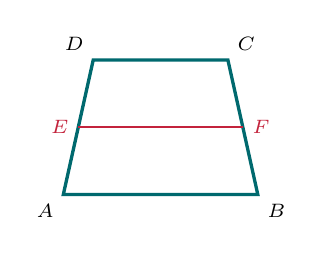
\begin{tikzpicture}[scale=0.95]
      \coordinate (D) at (0.4, 1.8);
      \coordinate (C) at (2.2, 1.8);
      \coordinate (A) at (0.0, 0.0);
      \coordinate (B) at (2.6, 0.0);
      \coordinate (E) at ($(A)!0.5!(D)$);
      \coordinate (F) at ($(B)!0.5!(C)$);
      
      \draw[very thick, color=brandNavy] (D) -- (C) -- (B) -- (A) -- cycle;
      \draw[thick, color=brandCrimson] (E) -- (F);
      
      \node[above left, font=\fontsize{7.5}{7.5}\selectfont] at (D) {$D$};
      \node[above right, font=\fontsize{7.5}{7.5}\selectfont] at (C) {$C$};
      \node[below left, font=\fontsize{7.5}{7.5}\selectfont] at (A) {$A$};
      \node[below right, font=\fontsize{7.5}{7.5}\selectfont] at (B) {$B$};
      \node[left, font=\fontsize{7.5}{7.5}\selectfont, color=brandCrimson] at (E) {$E$};
      \node[right, font=\fontsize{7.5}{7.5}\selectfont, color=brandCrimson] at (F) {$F$};
    \end{tikzpicture}
  \end{minipage}
\end{khboxorange}

\vspace{2pt}
\begin{multicols}{2}
  \noindent
  \begin{minipage}{\linewidth}
    \exhead{22} គេឱ្យចតុកោណព្នាយ $ABCD$ ដែលមាន $AB \parallel XY \parallel DC$ ។ បើស្គាល់ប្រវែង $AX = 3\text{dm}$, $XD = 8\text{dm}$ និង $BC = 9\text{dm}$ ។\\
    ចូរគណនាប្រវែង $BY$ និង $YC$ ។
    \begin{center}
      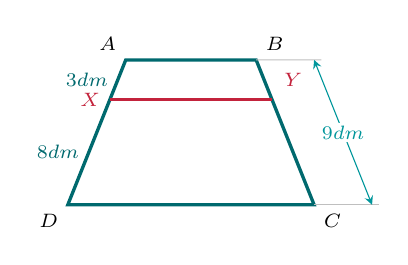
\begin{tikzpicture}[scale=0.92]
        \coordinate (A) at (0.8, 2.0);
        \coordinate (B) at (2.6, 2.0);
        \coordinate (D) at (0.0, 0.0);
        \coordinate (C) at (3.4, 0.0);
        \coordinate (X) at ($(D)!0.727!(A)$);
        \coordinate (Y) at ($(C)!0.727!(B)$);
        
        \draw[very thick, color=brandNavy] (A) -- (B) -- (C) -- (D) -- cycle;
        \draw[thick, color=brandCrimson] (X) -- (Y);
        
        \node[above left, font=\fontsize{7.5}{7.5}\selectfont] at (A) {$A$};
        \node[above right, font=\fontsize{7.5}{7.5}\selectfont] at (B) {$B$};
        \node[below left, font=\fontsize{7.5}{7.5}\selectfont] at (D) {$D$};
        \node[below right, font=\fontsize{7.5}{7.5}\selectfont] at (C) {$C$};
        \node[left, font=\fontsize{7.5}{7.5}\selectfont, color=brandCrimson] at (X) {$X$};
        \node[above right=1pt, font=\fontsize{7.5}{7.5}\selectfont, color=brandCrimson] at (Y) {$Y$};
        
        \node[left, font=\fontsize{7}{7}\selectfont, color=brandNavy] at ($(A)!0.5!(X)$) {$3\text{dm}$};
        \node[left, font=\fontsize{7}{7}\selectfont, color=brandNavy] at ($(X)!0.5!(D)$) {$8\text{dm}$};
        
        % Clean offset dimension line for BC
        \draw[gray!50, line width=0.3pt] (B) -- (3.5, 2.0);
        \draw[gray!50, line width=0.3pt] (C) -- (4.3, 0.0);
        \draw[<->, >=stealth, color=brandBlue, line width=0.4pt] (3.4, 2.0) -- (4.2, 0.0) node[midway, fill=white, inner sep=1pt, font=\fontsize{7}{7}\selectfont] {$9\text{dm}$};
      \end{tikzpicture}
    \end{center}
  \end{minipage}

  \columnbreak

  \noindent
  \begin{minipage}{\linewidth}
    \exhead{23} ក្នុងត្រីកោណ $ABC$ គេមាន $DE \parallel AB$ ។ ចូរបំពេញប្រវែងដែលបាត់ក្នុងតារាងខាងក្រោម ៖\\[3pt]
    \begin{center}
      \renewcommand{\arraystretch}{1.26}
      \begin{tabular}{|c|c|c|c|c|c|c|}
        \hline
        \rowcolor{koreaTeal!25}
        \textbf{ល.រ} & $AD$ & $DC$ & $AC$ & $BE$ & $EC$ & $BC$ \\
        \hline
        \khlabel{ក} & $3$ & $2$ & $5$ & $6$ & \textbf{...} & \textbf{...} \\
        \hline
        \khlabel{ខ} & $7$ & $3$ & \textbf{...} & \textbf{...} & $5$ & \textbf{...} \\
        \hline
        \khlabel{គ} & $2$ & \textbf{...} & \textbf{...} & $3$ & $4$ & \textbf{...} \\
        \hline
        \khlabel{ឃ} & \textbf{...} & $8$ & $20$ & \textbf{...} & \textbf{...} & $15$ \\
        \hline
        \khlabel{ង} & $12$ & \textbf{...} & $30$ & $9$ & \textbf{...} & \textbf{...} \\
        \hline
      \end{tabular}
    \end{center}
    \vspace{2pt}
    \begin{center}
      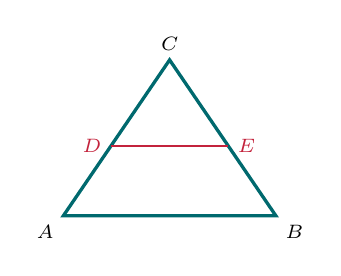
\begin{tikzpicture}[scale=0.90]
        \coordinate (C) at (1.5, 2.2);
        \coordinate (A) at (0.0, 0.0);
        \coordinate (B) at (3.0, 0.0);
        \coordinate (D) at ($(C)!0.55!(A)$);
        \coordinate (E) at ($(C)!0.55!(B)$);
        
        \draw[very thick, color=brandNavy] (C) -- (A) -- (B) -- cycle;
        \draw[thick, color=brandCrimson] (D) -- (E);
        
        \node[above, font=\fontsize{7.5}{7.5}\selectfont] at (C) {$C$};
        \node[below left, font=\fontsize{7.5}{7.5}\selectfont] at (A) {$A$};
        \node[below right, font=\fontsize{7.5}{7.5}\selectfont] at (B) {$B$};
        \node[left, font=\fontsize{7.5}{7.5}\selectfont, color=brandCrimson] at (D) {$D$};
        \node[right, font=\fontsize{7.5}{7.5}\selectfont, color=brandCrimson] at (E) {$E$};
      \end{tikzpicture}
    \end{center}
  \end{minipage}
\end{multicols}

\end{document}
